\input{preamble}
\pretitle{\begin{center} \fontsize{20}{20} \usefont{OT1}{phv}{b}{n} \selectfont}
	\title{Cybernetic Augmentation - a Key to Utopia or Dystopia?}			  
	% Title of your article goes here
	
	\posttitle{\vspace{7pt} \par {\Large WM0324LR Ethics Essay 2014-2015} \end{center} \vspace{0.1cm}}



\preauthor{\begin{center} \lineskip 0.1cm }
	\author{Seong Hun Lee 4145623, Manan Siddiquee 4185692}										% Author names go here
	\postauthor{\end{center}} % Change your group name!

 \date{}																	% Do not show date in \maketitle command


%%% Begin document
\begin{document}
	\twocolumn[\begin{@twocolumnfalse}
		\maketitle
		
		\begin{abstract}
		\noindent																% Remove default indentation
		\textbf{ \\ Here goes the abstract \\}
		\end{abstract} 
		\vspace{0.5cm}
		
	\end{@twocolumnfalse}]

	%% The sections
	\section{Introduction} 
	%Our biggest defining characteristic as human beings is our intellect. Needless to say we are not the strongest, the fastest or the most resilient to change that nature has to offer. Still we populate most of the biomes of this world and consciously define our lives and our habitats like no other animal on Earth. All of this in spite of our frailty compared to what nature has to offer, and all of this due to the only advantage that nature gave us; our ability to think better than any other animal that we know of.

%The source of the prosperity that humans have achieved in the last few millennium is the ability to make tools to complement ourselves; we have made tools to adapt the environment more habitable, ensured our food supply, increased our strength and dexterity, widened our knowledge and improved our ability to carry out mental activities. However, after the  millennium of progress we are approaching a new dimension of technology; a dimension which some believe will be our salvation while others would easily relate to the legends of Icarus, Pandora’s box and Prometheus’ fire. The dimension referred to is the prospect of actively and intrusively improving the human mind and body. Developments in fields such as electronics, nanotechnology, robotics, cybernetics, information technology, neurotechnology, genetic engineering and pharmacology, among others, are enabling a new field of technology labeled by some as ‘Human Engineering’ to emerge.

Humanity's ability to make tools to complement itself can arguably be the most important contributor to its success over the last few millennia; we have made tools to adapt the environment to our needs, ensure our food supply, increase our strength and dexterity, widen our knowledge and improve our ability to carry out mental activities. However, after millennia of progress we are approaching a new dimension of technology; a dimension which some believe will be our salvation while others think it will be our undoing. The dimension referred to is the prospect of actively and intrusively improving the human mind and body. Developments in fields such as electronics, nanotechnology, robotics, cybernetics, information technology, neurotechnology, genetic engineering and pharmacology, among others, are enabling a new field of technology labelled by some as ‘Human Engineering' to emerge.

The authors of this paper realize that human engineering is a very broad and trans-disciplinary field, and it would take volumes to analyse its ethical implications; thus this paper attempts to narrow the field by only looking at the ethical implications of one form of ‘Human Engineering’; namely cybernetic human augmentation. For the purpose of this paper cybernetic human augmentation is defined as the following: any (1) electro-mechanical addition to the human body that (2) becomes a natural part of the human body and that (3) improves the performance of an individual beyond normal human capacities. Needless to say genetic or chemical forms of human augmentation are external to the purview of cybernetic augmentation. Also, another important remark should be made that the scope of cybernetic human augmentation defined in this paper deals with the enhancement of the human capability "beyond the statistically normal standard", and therefore it does not consider the therapeutic use of the technology (e.g. prosthetic limbs for the amputees, artificial eyes/ears for the blind/deaf, memory chip for the patients suffering from Alzheimer's disease, etc.). Although there are complications for making this divide between therapy and enhancement, they will also be considered external to the scope of this paper.

The paper is structured as follows; the first part of the essay looks at the effects of cybernetic human augmentation on society; following this an ethical perspective is used to analyse the effects of augmentation. After looking at the effects and their ethical implications, recommendations are made to support the implementation of cybernetic augmentation on society. Finally, the conclusions are drawn regarding the viewpoints and approaches towards cybernetic augmentation, its ethics and its effects on the future of humanity.
	\section{Analysis}
    To explore the potential ethical implications of cybernetic augmentation in a more structured manner, a distinction is made between the two types of cybernetic augmentations: 
\begin{enumerate}
	\item Augmentations to enhance the user's physical ability
	\item Augmentations to enhance the cognitive ability.
\end{enumerate}
For example, if one's arm is replaced by a robotic arm which gives the user a superior arm with better strength and agility, then it is seen as an augmentation which enhances the physical ability. On the other hand, if a computer chip is implemented in one's brain to increase the user's memory capacity, then it is considered as an augmentation which enhances the cognitive ability of the user. 

With such a distinction in mind, let us analyze and discuss the ethical implications of cybernetic augmentation. Before we start, it is important to ask ourselves "What is meant by an ethical implication?". According to the Longman Dictionary of Contemporary English, an implication means "a possible future effect or result of an action, event, decision, etc" \cite{Longman_dic}. Therefore, an ethical implication would mean the possible future effect or result with regard to associated moral values and principles of morality. For analysis, this can be viewed as divided into two main aspects: namely, the potential benefits and risks. Therefore, in this section, the potential benefits and risks of the cybernetic augmentation are contemplated and discussed.

% Manan(14-12-2014 1636): The division of ethical implications to potential benefits and risks is flawed i think. ethics has to do with whats right and wrong, not what is beneficial or harmful per se. a beneficial thing can be wrong based on values and vice versa.

    \subsection{Benefits of cybernetic augmentation}

There can be numerous potential benefits when the cybernetic augmentation is implemented to enhance the user's physical and/or cognitive ability. In this essay, some of the main benefits of cybernetic augmentation are considered and discussed. Certain technologies are mentioned as examples to illustrate these benefits; the authors realize that these technologies can easily be risks, however in this part of the discussion only the prospective benefits are mentioned. The benefits are: ease hardships, improve health and survivability, create new opportunities, improve safety and welfare, improve efficiency and create happiness. Of course, there will be many other unmentioned potential benefits (and risks), but it should be noted that our intention is to give an overview and "food for thought" that is useful and adequate to comprehend the general implications, rather than to give you an exhaustive list of every possibility in the future. 

{\bf (1) Ease hardships} \\ 
One way that the cybernetic augmentation can be used to achieve the sense of better well-being is by enabling the users to carry out their daily actions in a more convenient way. For example, with augmented arms or legs, one may never have to struggle when lifting or carrying things. Also, the level of pain might be controlled in those augmented organs - for example, when you touch something very cold or hot beyond a certain threshold level, then it may regulate the synaptic information to your nerve system that you do not feel the pain you would have felt if you were not augmented. Such technology of physical cybernetic augmentation can give the user more control over their bodies, and thus reducing the level of inconvenience and stress. Furthermore, one can also consider the use of sensory/cognitive augmentation, such as an augmented eye which enables the user to see clearly during night with little light; this may be done by modifying or improving visual prosthesis devices {\bf CITE TO VISUAL PROSTHESES FOR BLIND}. Another kind of cognitive augmentation can be a computer chip that can be implemented in the brain to enhance the memory capability {\bf CITE TO NEURAL PROSTHESIS BERGER ET AL}. Such technology of cognitive cybernetic augmentation can lead to the better perception and management of the daily-life information.

{\bf (2) Improve health and survivability} \\
Since cybernetic enhancements will enhance the mind and the body of the person in question, it can be argued that their chances of survival will increase. A stronger, smarter person will be able to handle herself better in case of dangers such as natural disasters or accidents. In addition, the cybernetic augmentation can help the users maintain or improve their health by incorporating advanced medical technology. For example, the research is ongoing on the development of the nanorobots which are designed to navigate through our bodies' blood vessels, detect cancerous cells, and kill them \cite{nanorobot}. Through the technology of cybernetic augmentation, such nanorobots can monitor our body more comprehensively, and perform medical tasks more quickly and efficiently at an early stage. 

{\bf (3) Create new opportunities}\\
Imagining further into the future, cybernetic augmentations may give us the ability to inhabit currently uninhabitable environments; for example, underwater or other planets with hazardous environments. Also, enhancements may lead to the creation of newer jobs and professions; the tasks which are considered as currently impossible or very difficult may become practicable when a workforce with enhanced ability are engaged. Additionally, once the cybernetic augmentation becomes an active trend of the society, there will be more initiatives for the further research, development and application of the technology in the fields of not only in cybernetic augmentation, but also in other fields of technology and industries.

{\bf (4) Improve safety and welfare}\\
Cybernetic augmentation will improve safety beyond the discussed health and physical improvements of the individual. Society will be physically and psychologically better equipped to deal with its problems. Society will have a stronger physical presence with improved capacities of the armies and police forces; psychologically our society will be better equipped as our leaders will have enhanced minds which will improve their faculties to solve social and political problems {\bf CITE TO BOSTROM AND ROACHE}. We can also increase safety and moral behaviour of users of cybernetic augmentation by incorporating safety and morally right decision making processes or fail safes in the augmentations. As an example imagine cognitive augments which informs the user of locations of rubbish cans if he needs to dispose of some waste; the 'moralization of technology' will be easier and more effective {\bf CITE TO Achterhuis, 1995 AS IN ETHICS BOOK PG 172}.

{\bf (4) Increased efficiency and productivity} \\
Enhanced physical capability of the workers by means of cybernetic augmentation is most likely to increase the efficiency and productivity of humanity. Humanity will be able to better optimize and specialize its manpower, meaning as a sum effect we will get more done. Augmentations can be doctored to suit the professions of individuals; for example, construction workers can get physical augmentation that make them stronger, miners may consider improving their lungs to filter out harmful pollutants, businessmen can consider neural implants that will keep his mind connected to important information networks.

{\bf (5) Create happiness} \\
Although it can be argued that the cumulative effect of the aforementioned benefits will be a general increase, the authors wish to assert that cybernetic augmentation in and of itself can be a source of greater happiness. Besides the obvious improvement to self image from being able to do more, people maybe able to use cybernetic augmentation to fulfil lifelong dreams that were previously unattainable; for example, someone with physical augmentations, wishing to scale mountains but with no previous experience will be safely able to do so. Cognitive augments can monitor the brain for depressive thoughts pattern and attempt to alleviate them for the user by suggesting her activities or providing more context for the sadness by referring to the arts, thereby allowing her to cope better. As extreme cases, neural implants may allow the user to experience a virtual reality or even directly stimulate parts of the brain that make people feel happy.



%Another view with respect to the well-being is that cybernetic augmentation can positively affect the users not only physically, but also psychologically, as the extra abilities can plausibly help them gain higher self-esteem and confidence. In particular, for those people with the psychological complex about certain parts of their body, or abilities which they feel inferior themselves, the cybernetic augmentation could be used to overcome such complexes and give them more sense of happiness and better well-being.

    \subsection{Potential risks}
Just like any other technology, the cybernetic augmentation has a double-side of ...........What are the potential risks of cybernetic augmentations which are implemented to enhance the user's physical and cognitive ability? 

\subsubsection{Risks of physical CA}
This is the risks of CA physical

\subsubsection{Risks of cognitive CA}
This is the risks of CA cognitive
    \subsection{Application of ethical theories towards cybernetic augmentation}
The main ethical issue that the introduction of cybernetic augmentation technology imposes on the society can be viewed in two different (but closely related) approaches: (1) an approach to deal with the ethical aspects of the technical risks by analyzing whether or not such risks are acceptable, and (2) an approach of duty ethics or virtue ethics which judges the act of cybernetic augmentation itself by directly relating to the moral values, such as human dignity. In the following sections, the two approaches are elaborated so as to discuss the ethical implications of cybernetic augmentation.

%the way i see it approach 1 is mills utilitarianism with more details. because the most relevant one seems a risk-benefit analysis.

\subsubsection{Analysis of the acceptability of the risks}
According to \cite{Ethics_textbook}, a risk can be considered morally acceptable only after considering the following aspects:
\begin{enumerate}
	\item The degree of informed consent with the risk
	\item The degree to which the benefits weigh up against the risks
	\item The availability of alternatives with a lower risk, and
	\item The degree to which risks an advantages are justly distributed (among the people)
\end{enumerate}

First of all, the principle of informed consent states that the potential risks and benefits must be fully informed to the people who might be influenced by the activity, and if they all agree to take the risks, then the risk can be considered morally acceptable. This is based on the freedom principle which respects the moral autonomy of the individuals and suggests that everyone is free to strive for his/her own pleasure, as long as there is no harm to others \cite{Ethics_textbook}. This alone however cannot become the sole criterion for judging the acceptability of risks because it is practically impossible to get consents from every individual who is influenced by the technology. As shown in the previous section, the potential risks of cybernetic augmentation exist not only towards the direct users, but also on the general society in the long term. It therefore becomes impractical to ask for consents from everyone. Moreover, considering the fact that the cybernetic augmentation technology is a newly emerging field, it is very difficult to fully comprehend the potential risks beforehand. 

The second consideration is the use of risk-cost-benefit analysis. This is based on the idea of utilitarianism (i.e. a type of consequentialism based on the utility principle which strives for the greatest happiness for the greatest number). Such approach can be useful as it can give us an intuitive idea on the overall impacts of the activity. It is for this reason that the potential benefits and risks are discussed in the previous section. However, one should be careful to avoid the fallacy of pricing (i.e. expressing every value in monetary terms) and realize that the implication of the cybernetic augmentation technology is multidimensional.

The third criterion for the acceptability of the risk are rather subtle in this case, as this paper focuses on the evaluation of the technology itself, rather than an engineering problem which strives to solve an existing problem. 

The last consideration to be taken into account is whether the risk and benefits are evenly distributed among the people. As discussed in the previous section, it is predictable that the rich will enjoy the benefits of cybernetic augmentation more, thereby causing an inequality issue. Nevertheless, it is also assumable that the users of cybernetic augmentation in the earlier phase of the development would take more risks than the users  in the later phase of the development where the application of technology has improved with more maturity.

All in all, it can be reasoned that the acceptability of the risk of cybernetic augmentation should not be judged based only on each criterion that is mentioned, but also through the continuous reflection and multidimensional considerations during the process of development and deployment of the technology.

\subsubsection{Duty ethics or Virtue ethics approach}
Whereas the analysis of the moral acceptability of the risks appears to be rather existentialistic, the approach from a duty ethics or virtue ethics allows us to consider a different aspect of the issue - Is cybernetic augmentation virtuous? Does it deteriorate moral values, such as human dignity? Is it the right thing to do? 

If 

%Instead, one should be aware of the fact that such ethical issues are often very abstract and subjective, as it directly deals with the moral values of the people which is reflected on the zeitgeist of the society. 

%One may dispute against this perspective by using an analogy to other currently available technology (e.g. "The cars enabled us to move faster, and the computers allowed for better management of information. No one says cars and computers damage our human dignity. The same should go for cybernetic augmentation." However, such argument is again subject to disputes as the cybernetic augmentation takes an intrusive form and becomes "as if it was a natural part of the human body". Therefore, the analogy between the cybernetic augmentation and currently existing technologies is not perfectly justifiable.

% % % NOTES

% technology assessment, collinridge dilemma,CTA; pg 32 ch1
% maybe some kind of talk about responsibility ch1 & 8
% Ethhical principles for engineers in a global environment (Luegenbiehl,2010); pg 55 ch2
% quote no harm principle and freedom principle when used subsubsection of acceptability of risk; pg74-5 ch3 ethics book
% use concepts of distributive justice and marginal utility; pg 76 ch3, ethics book
% use the concept of eudamonia from aristotles vitue ethics; pg 84 ch3, ethics book
% issue of the slipperly slope argument as in some paper i read; issue of similarity to the following quote if we choose for CA 'Vaughan’s analysis of the Challenger disaster illustrates a more general point: decisions – also incremental and implicit ones – tend to commit us to certain courses of actions and frame subsequent decisions (Darley, 1996).' pg 145 ethics book
% ethics during approach to design i.e. responsibility of researchers and designers; problem of 'radical design concept in CA, this maybe part of risks aswell. ch 6;
% technological mediation, moralizing of technology ch 7. moralizing of tech mentioned in benefits part
% strong presence of both uncertainity and ignorance in CA, the ignorance can be more conseuquential. this point maybe more appropriate in risks part ch 8





 %    \subsection{Physical Cybernetic Augmentation}

For this essay physical cybernetic augmentation is defined as any kind of cybernetic augmentation that enhances the physical (i.e. of the body) qualities of a human being. Examples of physical improvement include among others an enhancement of physical strength, giving human beings gills and webbed feet to adapt for life underwater or improving the lungs and skin so that human beings can tolerate different types of atmospheres.

\subsubsection{Benefits of Physical CA}

There can be numerous potential benefits when the cybernetic augmentation is implemented to enhance the user's physical ability. For example, these are: better well-being, increased efficiency and productivity, self-defense, further development of technology. Of course, there will be many other unmentioned potential benefits (and risks), but it should be noted that our intention is to give an overview and "food for thought" that is useful and adequate to comprehend the general implications, rather than to give you an exhaustive list of every possibility in the future. 


{\bf Better well-being of the user} \\
Among the various potential benefits of the physical cybernetic augmentation, the most apparent beneficiaries would be the amputees (i.e. those who lost their limb due to accident, war, etc.) and patients with physical disability. The cybernetic augmentation can plausibly allow those people to move and look like a normal person again, and moreover, it can give them extra physical abilities beyond the normal standard level. Besides, this can affect them not only physically, but also mentally; they can gain higher self-esteem and confidence, which would give them more sense of happiness. 

Moreover, just an average people can also enjoy the sense of better well-being as the cybernetic augmentation can enable them to carry out their daily actions in a more convenient way. For example, with augmented arms or legs, one may never have to struggle when lifting or carrying things. Also, the level of pain might be controlled in those augmented organs - for example, when you touch something very cold or hot beyond a certain threshold level, then it may regulate the synaptic information to your nerve system that you do not feel the pain you would have felt if you were not augmented. Such technology can give the user more control over their bodies, and thus reducing the level of inconvenience and stress.

In addition, the cybernetic augmentation can help the users maintain or improve their health by incorporating advanced medical technology. For example, the research is ongoing on the development of the nanorobots which are designed to navigate through our bodies' blood vessels, detect the cancerous cell, and kill it \cite{nanorobot}. Through the technology of cybernetic augmentation, such nanorobots can monitor our body more comprehensively, and perform medical tasks more quickly and efficiently at an early stage. 

Such strengths gained by the cybernetic augmentation are likely to increase the chance of the user's survival in wild nature (or in the unfamiliar environment or situations) as this technology can possibly allow him/her to evolve into a stronger and more adapted species. 

{\bf Increased efficiency and productivity}\\
An enhanced physical capability of the workers by means of cybernetic augmentation is most likely to increase the efficiency and productivity of the work and industry. This would be a good news to the employers, since they can either reduce the labor cost by employing less number of people to do the same job, or increase the profits with the same number of employees because the they would have enhanced efficiency and productivity, thanks to cybernetic augmentation.

{\bf Self-defense and military application}\\
One may claim that cybernetic augmentation which enhances the physical ability would lead to more security as it can be used as means of self-defense. However, this is indeed subjected to the dispute that it can be used also as a weapon to attack others, which is analogous to the current debate regarding the gun control issue in U.S. Nevertheless, it is hard to deny that the cybernetic augmentation can be used to enhance the level of self-defense of the user, compared to the non-users of cybernetic augmentation.

Such advantage of cybernetic augmentation can be most extensively exploited in the field of military application; the soldiers with high-level cybernetic augmentation can gain enhanced physical combat ability.

{\bf Further development of technology}\\
Once the physical cybernetic augmentation becomes an active trend of the society, there will be more initiatives for the further research, development and application of the technology in the fields of not only in cybernetic augmentation, but also in other fields of technology and industries. For instance, the design of the interfaces of many electronic gadgets or machines can change into a more efficient form (e.g. semi-automated guns that can be attached to the part of an augmented arm, or infrared monitors/screens when the visible frequency of our eyes can be controlled using an advanced electronic lens, etc)


\subsubsection{Risks of Physical CA}

\begin{itemize}
	\item Short-term risks that may harm the bodies and decrease convenience
	\item Unknown psychological effect
	\item Increased life expectancy has side effects: over population increased social-welfare cost, youth unemployment, etc.
	\item Increased sense of insecurity (Analogous to gun control issue)
	\item Employment issue (i.e. few people replacing many people's job)
	\item Military application can be problematic in view of ethics
	\item Necessity to change many regulations and laws, as well as to create ones
	\item Inequality issue
	\item Human dignity - loss of "humanness"
	
\end{itemize}
 %    \subsection{Cognitive Cybernetic Augmentation}

There are three primary types of cognitive enhancements that can be attained through cybernetics. 1. improvement of thinking capacity; 2. improvement of sensory capacities; 3. accommodation for a interfacing with the external world. Current innovations have only began to scratch the surface of devices that may lead to the second or third type of enhancements. Most of the devices being researched are not intended for enhancement rather aiding people with existing mental or physical disabilities; however, one need only apply a little imagination to see how the application of these technologies to people without illness or disabilities may lead to enhancements of their functionalities.

{\bf Available technology}

Currently no form of cybernetic technology exists that can supplement the thinking capacity of the bearer. However some experiments on animals have had promising results. The Prosthetic Neuronal Memory Silicon Chips designed by Theodore Berger {\bf C} have been demonstrated to be able to restore memories in rats and monkeys. Although he has not been able to form long term memories with his chip, he believes that his research will eventually lead to devices capalble of doing so. He hopes these these devices will be able to help people with Alzheimer's disease, stroke or brain injury that suffer from memory loss.

Cochlear implants {\bf C} are devices which directly interface with the nerves connecting the ear and the brain to give severly deaf people a sensation of sound; these devices are examples of cybernetic devices augmenting sound sensations. Devices such as the Argus II {\bf C} and Alpha IMS {\bf C} are implants placed directly within the retina of a person suffering from vision loss due to inability of the retial cells to detect light. These implants are stimulated either by processing the image externally in the case of Argus II or by the directly by the light entering the eye, which are than converted to electronic impulses by the implants and sent to the brain. 

Examples of existing devices for interfacing between the brain and an external object range from simple, wearable and off the shelf EEG devices such as Emotiv {\bf C} and iFocusBand {\bf C} to expermental devices that physically interfaces with the brain using electrodes such as BrainGate {\bf C}. While the former is mostly used for recreational purposes, the latter is being researched and developed to give people physically disabled some means of communicating with the world. Researchers at MIT are working on a device {\bf C}, which is at a very early stage of development, that plans to fully bypass the eye and send impulses directly to the brain to give its user some kind of vision.


{\bf Prospective technology}

With the knowledge of the current innovations that are already available and the ones expected to be available to us in the near future, one may speculate as to the kind of cognitive enhancement technology that humanity may have in the far future.

In lieu with the devices of Theodore Berger {\bf C} one can imagine a range of devices that will aid and supplement the memory of human beings to beyond human levels. Science fiction writers and futurists have speculated on a device which they are calling an exocortex {\bf C}; this external cortex will supplement our current conciousness by adding more memory, processing power, system software and interfacing ports.

Due to the wide range of electical sensors that we have available, the possibilities of sensory augmentation are vast. One can augment the human vision to see a much wider range of the electromagnetic spectrum; The same can be done with hearing, tasting, smelling or even feeling. On a more imaginative and abstract note, sensory devices could be used to transpose different sensation onto different ones. If we connect our auditory devices to the visual perceptions, we may be able to see sounds, or hear the sensations of feeling and tasting.

Although any kind of cybernetic device implies some kind of interfacing between mind and machine; however here machine means an object existing outside the body. Already the exocortex mentioned earlier hinted to some kind of interfacing, however purely interfacing cybernetic devices would also be a possibility. One may have a device that just links her/his mind to the internet, or to a network of other minds using those devices. Such a device maybe used by the wearer to communicate with other devices such as his car or his 'smart' house. \\

{\bf Ethical implications}

The ethical implications of such cognitive enhancements have been listed here. In the final essay few of these issues will be focused upon and elaborated upon.

\begin{enumerate}
    \item Risk to humanbody, humanity and way of life
    \item Affordability leading to human segregation and social startification (violation of utilitarian ethics)
    %\item Different classes of humanity with different rights (rethinking of basic human rights)
    \item Communicatability between two types of sensory enhanced human
    \item Need for rethinking of most institutions; e.g. having memory chips would nullify most academic tests we have now.
    \item Manipulation of memory which maybe argued as fundamental to the fabric of human character formation (violation of virtue ethics; barrier to eudamonia)
    \item Misuse of this technology; potential harm that humanity can unleash on itself with these enhancements. This may express itself as the following (violation of duty ethics):
        \begin{itemize}
            \item Mind reading
            \item Potential hacking of other human beings
            \item Misuse by the government; e.g. with interrogation, monitoring of citizens thoughts, or altering their personality
        \end{itemize}
\end{enumerate}

    \section{Authors' Opinions and Recommendations}
    Despite a multitude of identified technical risks and ethical concerns, the authors of this paper claim that the emergence and development of the CA should not be simply avoided, but should rather be encouraged in such a manner that the moral autonomy of those who are willing to utilize the technology is respected while the possible risks are striven to be minimized. Moreover, we argue that an excessively conservative view which tries to indiscreetly restrict the entire human augmentation technology itself will not only hinder the gateway to the great benefits of the technology, but also limit the possibility to develop a more encompassing social, economical, technological, and ethical framework which would help us better comprehend the implications of the related technologies and allow us to deal with the risks more effectively.

As a way of utilizing the technology while minimizing the technical risks and ethical concerns, the authors propose the following recommendations:
\begin{itemize}
	\item Active encouragement of the application of CA technology for therapeutic purpose (e.g. prosthetic limbs for the amputees illustrated in Figure \ref{prosthetic_arm}, and visual prostheses for the blind illustrated in Figure \ref{prosthetic_eye}). Since such kind of use of the technology is much less controversial, it is recommendable that the development of the augmentation technology be focused on these medical fields for the time being. Once the technology gains more maturity and people become more familiar (and knowledgeable) with it, we can then have more meaningful discussions concerning the acceptability of the CA technology that is intended to enhance the human ability "beyond the normal level".
	\item Active encouragement of the development of non-permanent/wearable cybernetic devices, starting from the smallest scale. If the intrusive nature of the CA is removed, there will be much less technical risks and ethical concerns. Therefore, it can be a great stepping-stone for the introduction of the CA technology for the similar reasons as in the previous item. 
	\item A discussion as to whether the CA is a key to Utopia or Dystopia can be meaningful as long as the discussion actively continues throughout the development and deployment of the technology, whilst refraining from making hasty conclusions (i.e. slippery slope fallacy). Note that CA is a very broad technology. Therefore, instead of judging the final possible outcome of the entire concept of the technology, one should rather try to find specific fields and aspects in which the technology can be applied with the highest acceptability. 
\end{itemize}

\begin{figure}[H]
	\centering
		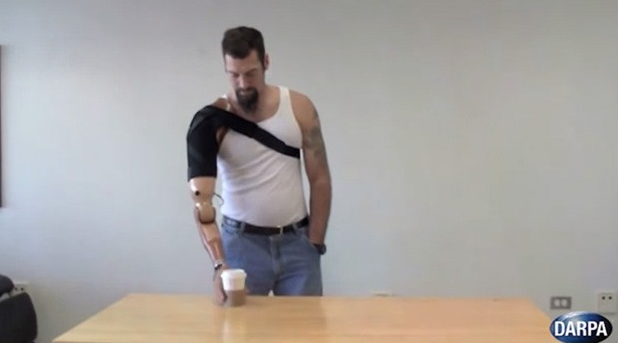
\includegraphics[width = 8cm]{prothesis_arm}
	\caption{Prosthetic arm developed by DARPA. An artificial arm is connected to the user's existing muscles and nerves\cite{prosthetic_arm}}
	\label{prosthetic_arm}
\end{figure}

\begin{figure}[H]
	\centering
	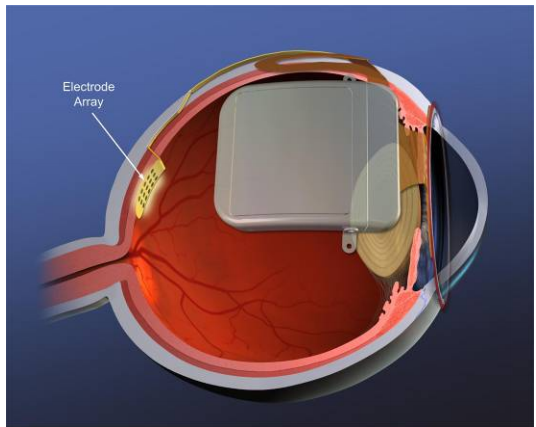
\includegraphics[width = 6cm]{prothesis_eye}
	\caption{Prosthetic retinal implant concept illustration \cite{retinal_implant}}
	\label{prosthetic_eye}
\end{figure}
    \section{Conclusions}
    This essay has attempted to briefly discuss what CA may mean for the future of humanity. It has firstly discussed the five potential benefits and five risks of CA. It than moved on to apply three normative ethical theories to analyse the morality of CA; the analysis found that utilitarianism can be used to justify CA if implemented correctly, duty ethics may face some difficulties with CA due to its rigid nature and finally that virtue ethics can be guiding principle for a positive implementation and application of CA in society. However, the ethical discussion revealed some pitfalls associated each ethical theory is present when implemented for CA, thus a pragmatic application of all three theories need to be made to obtain a just and fair ethical code for CA.

Finally some recommendations were made about the humanity's approach towards CA. It is the belief of the authors that CA is something that we will need to deal with; conservatism will not only hinder progress, it will handicap our ability to control the development of CA and implement policy and framework to regulate to lead to the greatest human good. Emphasis was put into both a gradual and thought development process as well as a slow exposure of this technology to the public. These would be pivotal in the way CA pans out in the future because having a slow and careful development process in parallel with a slow step wise public exposure of the technology will allow the developers to better understand the consequence of the technology and leave time for ancillary institutional and policy frameworks to develop. Better understanding of the technological consequences as well as an accommodating framework will guide this technology so that it can lead us closer to a utopia and make sure it does not implode causing a dystopia.

\bibliographystyle{plain}
\bibliography{mybib}
	
\end{document}

